\documentclass{article}

\title{Comparing Mechanistic and Statistical Models to Forecast Influenza in the U.S.}

\author{Logan Brooks, Spencer Fox, Craig McGowan, Sasikiran Kandula, \\ Dave Osthus, Evan Ray, Nicholas G Reich, Roni Rosenfeld, Jeffrey Shaman, \\Abhinav Tushar, Teresa Yamana [authorship list to be finalized]}

\usepackage[letterpaper, margin=1in]{geometry} % margin
\usepackage{lineno}% add line numbers
\usepackage{graphicx}
\usepackage[colorlinks=true, allcolors=blue]{hyperref}
\usepackage{parskip}        % for spacing after paragraphs http://ctan.org/pkg/parskip
\usepackage{url}            % simple URL typesetting
\usepackage{booktabs}       % professional-quality tables
\usepackage{amsfonts}       % blackboard math symbols
\usepackage{nicefrac}       % compact symbols for 1/2, etc.
\usepackage{amsmath, amsfonts}
\usepackage{setspace}
\linenumbers % line numbers
\onehalfspacing



% For computer modern sans serif
\usepackage[T1]{fontenc}
\renewcommand*\familydefault{\sfdefault} %% Only if the base font of the document is to be sans serif


\begin{document}

\maketitle

\tableofcontents

\section{Introduction}
Forecasts of infectious disease outbreaks can inform public health response to outbreaks. Close collaboration between public health policy-makers and quantitative modelers is necessary to ensure the forecasts have maximum impact and are appropriately communicated to the public and the broader public health community. 

Infectious disease modeling has proven to be fertile ground for statisticians, mathematicians, and quantitative modelers for over a century. Yet there is not a consensus on a single best modeling approach or method for forecasting the dynamic patterns of infectious disease outbreaks, in both endemic and emergent settings. Mechanistic models consider the biological underpinnings of disease transmission, and are in practice are typically implemented as variations on the Susceptible-Infectious-Recovered (SIR) model. Phenomenological models largely ignore the biological underpinnings and theory of disease transmission and focus instead on using data-driven, empirical and statistical approahces to make the best forecasts possible of a given dataset, or phenomenon. Both approaches are commonly used and both have advantages and disadvantages in different settings.   


\section{Methods}

\subsection{FluSight Challenge Overview}

Starting in the 2013-2014 influenza season, the CDC has run the "Forecast the Influenza Season Collaborative Challenge" (a.k.a. FluSight) each influenza season, soliciting weekly forecasts for specific influenza season metrics from teams across the world. These forecasts are displayed together on a website during the season and are evaluated for accuracy after the season is over.\cite{PhiResearchLab} 
Detailed methodology and results from this challenge have been published\cite{Biggerstaff2016}, but summarize the key features of the challenge here.

The FluSight challenge has been focused on forecasts of the weighted percentage of doctor's office visits for influenza-like-illness (wILI) in a particular region. This is a standard measure of seasonal flu activity, for which public data is available back to the 1997/1998 influenza season. During each influenza season, this data is updated each week by the CDC (Figure \ref{fig:timezero-schematic}). When the most recent data is released, the prior weeks' reported wILI data may also be revised. The unrevised data, available at a particular moment in time, is available via the DELPHI real-time epidemiological data API beginning in the 2013/2014 season.\cite{DELPHI} This API enables researchers to ``turn back the clock'' to a particular moment in time and use the data available at that time. This enables more accurate assessment of how models would have performed in real-time. 

\begin{figure}[htbp]
\begin{center}
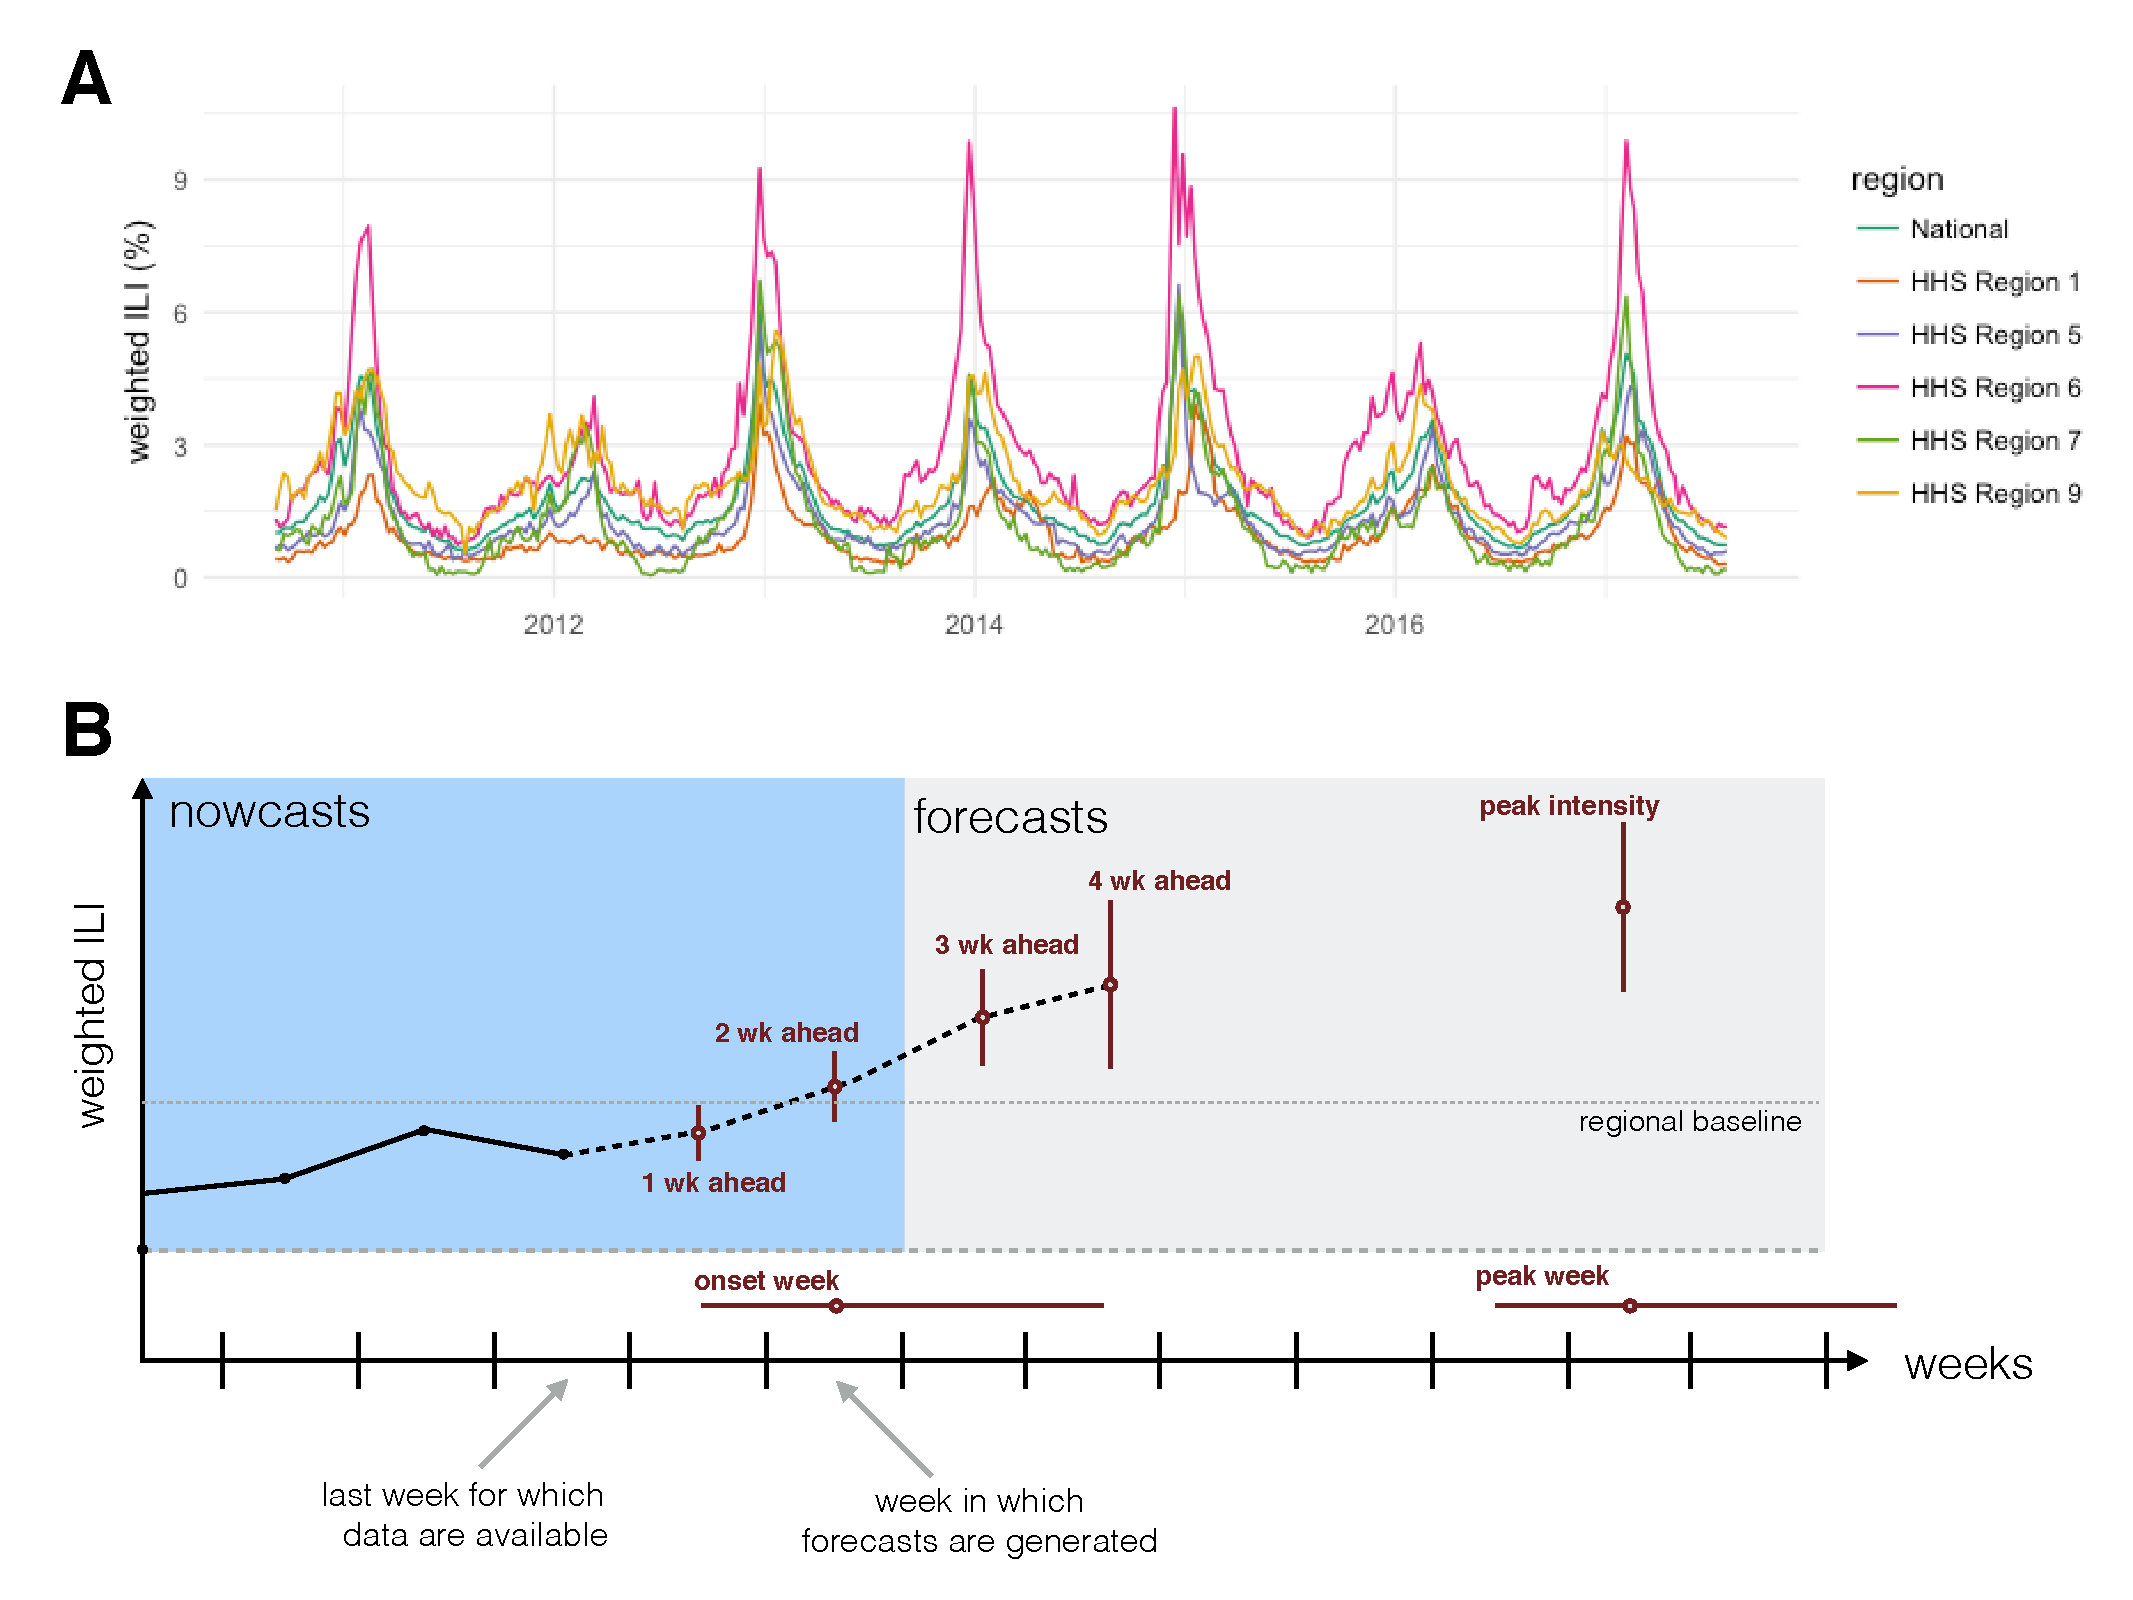
\includegraphics[width=\textwidth]{static-figures/timezero-sketch.pdf}
\caption{A schematic showing when data arrives in realtime relative to when the forecasts are made available.}
\label{fig:timezero-schematic}
\end{center}
\end{figure}


The FluSight challenges have defined seven forecasting targets of particular public health relevance. Three of these targets are fixed scalar values for a particular season: onset week, peak week, and peak intensity (i.e. the maximum observed wILI percentage). The remaining four targets are the observed wILI percentages in each of the subsequent four weeks. 

The FluSight challenges have also required that all forecast submissions and follow a particular format. A single submission file (a comma-separated text file) contains the forecast made for a particular epidemic week (EW) of a season. Standard CDC definitions of epidemic week are used. Each file contains binned predictive distributions for seven specific targets across the 10 HHS regions of the US plus the national level. Each file contains over 8000 rows and typically is about 400KB in size.

To be included in the model comparison presented here, previous participants in the CDC FluSight challenge were invited to provide out-of-sample forecasts for the 2010/2011 through 2016/2017 seasons. For each model, this involved creating 233 separate forecast submission files, one for each of the weeks in the seven training seasons.
Each forecast file represented a single submission file, as would be submitted to the CDC challenge. 
Each team created their submitted forecasts in a prospective, out-of-sample fashion, i.e. fitting or training the model only on data available before the time of the forecast (see Figure \ref{fig:timezero-schematic}). 

\subsection{Description of this Forecasting Experiment}


\subsection{Summary of Models}

Particular reference to the 2-3 models that can be considered ``baseline'' models:
 - Delphi-Uniform
 - ReichLab-KDE

%% Table with columns for:
%%   - institution
%%   - model name
%%   - underlying method
%%   - statistical/mechanistic
%%   - non-ILI data sources

\subsection{Metrics Used for Evaluation and Comparison}

Forecasts have historically been evaluated by the CDC using two metrics, the log-score and the mean absolute error. These two metrics capture different desirable features of performance. The log-score enables evaluation of both the precision and accuracy of a forecast, using the predicted density function.\cite{Gneiting2007} The absolute error provides an interpretable summary of the amount of error the point estimates had on average.\cite{Reich2016} 

We used a modified form of the log-score to evaluate forecasts, in line with the evaluation performed by the CDC. The log-score is defined as $\log f(\hat z|\bf{x})$ where $f(z|\bf{x})$ is a predictive density function for some target $z$, conditional on some data $\bf{x}$ and $\hat z$ is the observed value of the target $z$. In practice, each model $m$ has a set of log scores associated with it are region-, target-, season-, and week- specific, notated as $\log f^{(m)}_{r,t,s,w}(\hat z|\bf{x})$. We evaluated model performance based on the exponentiated average log scores, which has been called ``forecast skill'' and is equivalent to the geometric mean of the probabilities assigned to the eventually observed outcome. 
For example, the forecast skill for model $m$ and target $t$ would be calculated as
\begin{eqnarray}
 FS^{m}_{t} & = & \exp \left ( \frac{1}{N} \sum_{r,s,w} \log \hat f^{(m)}_{r,t,s,w}(\hat z|{\bf x}) \right ) \\
 & = & \left ( \prod_{r,s,w} \hat f^{(m)}_{r,s,w}(\hat z|{\bf x}) \right ) ^{1/N} 
\end{eqnarray}
where $N$ is the total number of log-scores for target $t$ and model $m$, across all combinations of region, season, and week. 
Further, within a given region-season-target combination, the weeks included in the calculation of the average forecast skill depend on when the onset and peak occur. Specifically, [[...]].
All weeks are included for the forecast skill calculations for the $k$-step ahead forecasts of wILI.

The log-scores are computed for the targets on the wILI percentage scale such that predictions within +/- 0.5 percentage points are considered accurate, i.e. log score = $\log \int_{\hat z -.5}^{\hat z + .5} f^{(m)}(z|{\bf{x}})dz$. For the targets on the scale of epidemic weeks, predictions within +/- 1 week are considered accurate, i.e. log score = $\log \int_{\hat z -1}^{\hat z + 1} f^{(m)}(z|{\bf{x}})dz$. 
\begin{itemize}
    \item log-score for predictive distribution, aggregated by (model), (model x season), (model x season x location), (model x season x target-type), (model x season x target), , (model x season x week)
    \item MAE for point predictions
\end{itemize}

\subsection{Formal comparisons of model performance}

\begin{itemize}
    \item permutation test for pairwise statistical comparison between two models
    \item beta regression or permutation test for comparison between groups of models (i.e. mechanistic vs. statistical)
\end{itemize}


\section{Results}

Things to confirm: removed weeks that CDC does not score, no onset seasons and multi peak years are handled appropriately

\subsection{Performance in forecasting week-ahead incidence}

\begin{itemize}
    \item describe historical model average performance and how it varies (min/max?) across seasons/regions and what that says about inter-season and inter-region variability
    \item what fraction of models did better than historical average/uniform.
    \item describe skill degradation has horizon increases
    \item 
\end{itemize}

\subsection{Performance in forecasting seasonal targets}

\begin{itemize}
    \item describe historical model average performance and how it varies (min/max?) across seasons/regions/targets
    \item what fraction of models did better than historical average/uniform.
    \item What is hard about Region 2?
\end{itemize}


\subsection{Characterize skill and variability in skill of each model}

TODO: make point plot of skill by season to show variability and average performance.

\begin{figure}[htbp]
\begin{center}
\includegraphics[width=\textwidth]{figures/fig-results-season.pdf}
\caption{Model results by season.}
\label{fig:results-season}
\end{center}
\end{figure}

\subsection{Performance of models by location}

Consider adding map that averages across all models, or shows max skill per region, as it varies quite a bit.

\begin{figure}[htbp]
\begin{center}
\includegraphics[width=\textwidth]{figures/fig-results-region.pdf}
\caption{Model results by region and target-type.}
\label{fig:results-region}
\end{center}
\end{figure}

\subsection{Performance of models by target}


\subsection{Performance of models by time-of-season}


\subsection{Comparison between statistical and mechanistic models}


\section{Discussion}

\subsection{Overview of key results and importance}
The first large-scale comparison of flu forecasting models from different modeling teams/philosophies across multiple years.

\subsection{Overview of statistical vs. mechanistic model comparison}
As our knowledge/data about the system mature, we expect mechanistic models to be better, but when true signals of mechanistic model is drowned out by observational noise or spatial aggregation, statistical models may perform better. This comparison serves as a barometer for where the current state of forecast models are.

\subsection{Limitations}

\begin{itemize}
    \item relatively few additional data sources incorporated
    \item no models that explicitly incorporate strain information
    \item no models with spatial information included
    \item seven seasons of data is not a lot (n=7) to draw strong conclusions about comparative model performance
    \item currently limited to models with only recent data...
\end{itemize}

\bibliographystyle{unsrt}
\bibliography{../flusightnetwork.bib}

\end{document}